Исходные тексты программы доступны в репозитории:\\
\url{https://github.com/CATSPDEs}

Комплекс программ для численного решения уравнений в частных производных разработан с использованием \texttt{C++11} (\texttt{Visual Studio 2015}, компилятор \texttt{MSVC}).

Для аналитических вычислений (расчёта локальных матриц и векторов, производных временного базиса и т.\,д.), оформления таблиц, рисунков и анимаций полученных решений использовалась мощная система символьной арифметики \texttt{Mathematica 10.4}.

\section{Стационарная задача}
\label{stationary}

Пусть дано уравнение\footnote{
	Уравнение вида $u_t - \nabla \cdot (a \, \nabla u) + r(u) = 0$ называют \textbf{уравнением диффузии--реакции} (\textit{diffusion--reaction eqn}). Слагаемое с оператором Лапласа «отвечает» за диффузию (или теплопроводность), зависящее от решения $u$ слагаемое --- за реакцию среды. 
	
	Если уравнение содержит конвективное слагаемое $q(\nabla u)$, то уравнение называют \textbf{уравнением конвекции--диффузии} (\textit{convection--diffusion eqn}).
	
	Если решение не зависит от времени ($u_t \equiv 0$) --- т.\,е. мы имеем дело со стационарной проблемой --- и $r(u) = c \, u - f$, то задача сводится к \textbf{стационарному уравнению диффузии--реакции} (\textit{steady--state diffusion--reaction eqn})~(\ref{eqn}).
	
	По этим причинами мы называем входящие в~(\ref{eqn}) функции $a$ и $c$ коэффициентами диффузии и реакции соответственно.  
}
\begin{equation}
	\label{eqn}
	- \nabla \cdot (a \, \nabla u) + c \, u = f, \quad \vect{x} \in \Omega,
\end{equation}
с краевыми условиями
\begin{equation}
	\label{BCs}
	- \vect{\hat{n}} \cdot (a \, \nabla u) = \kappa \, (u - g_D) - g_N, \quad \vect{x} \in \partial \Omega,
\end{equation}
где $\vect{x} \coloneqq (x, \, y) \in \mathbb{R}^2$~--- аргумент, $a$, $c$, $f$, $\kappa$, $g_D$ и $g_N$~--- заданные $\mathbb{R}^2 \rightarrow \mathbb{R}$ функции, $\Omega \subset \mathbb{R}^2$~--- отрытая область с кусочно--гладкой границей $\partial \Omega$, $\vect{\hat{n}} \: : \: \mathbb{R}^2 \rightarrow \mathbb{R}^2$~--- нормированный вектор, нормальный к $\partial \Omega$ и направленный вне области. 

Нужно найти решение $u = u(\textbf{x})$, удовлетворяющее~(\ref{eqn}~--~\ref{BCs}).

\subsection{Вариационная постановка}
\label{Galerkin}

Аналитическое решение задачи~(\ref{stationary}) на практике доступно редко --- оно может быть найдено для «ограниченного» набора входных в (\ref{eqn}~--~\ref{BCs}) функций и «простых» областей. Подробно аналитические методы решения уравнений в частных производных рассмотрены в~\cite{PDEs}.

Мы рассмотрим методы численного решения задачи~(\ref{stationary}) (в этой секции --- методом конечных элементов (МКЭ), в следующей --- связкой МКЭ и метода конечных разностей (МКР) для нестационарной задачи). 

Предположим\footnote{
	Зачастую функция $u$ интерпретируется как температура плоской области $\Omega$. Известно, что температура пропорциональна скорости движения частиц в точке $\vect{x}$: $u(\vect{x}) \propto V(\vect{x})$, $u^2(\vect{x}) \propto V^2(\vect{x})$. Принимая во внимание конечность кинетической энергии, можно утверждать, что 
	$$
		\infty > \int_\Omega u^2(\vect{x}) \diff{\vect{x}} \eqqcolon \normL{u}^2.
	$$
	Стало быть, пространство Лебега --- подходящее место жительства для искомого решения.
}, что решение задачи~(\ref{stationary}) живёт в гильбертовом пространстве 
\begin{equation}
\label{V}
	\mathbb{V} \coloneqq \{ v = v(\vect{x}): \normL{v} + \normL{\nabla v} < \infty \}.
\end{equation}

Домножим (в смысле скалярного произведения в $L_2$) уравнение~(\ref{eqn}) на тестовую функцию~$v~\in~\mathbb{V}$:
\begin{subequations}
\label{multByTestFunc}
	\begin{align}
		\int_{\Omega} f \, v \diff{\vect{x}}  
		&= 
		\int_{\Omega} - \nabla \cdot (a \, \nabla u) \, v \diff{\vect{x}}  + 
		\int_{\Omega} c \, u \, v \diff{\vect{x}}  \\
		&= 
		\int_{\Omega} a \, \nabla u \cdot \nabla v \diff{\vect{x}}  -
		\int_{\partial \Omega} \vect{\hat{n}} \cdot (a \, \nabla u) \, v \diff{s} +
		\int_{\Omega} c \, u \, v \diff{\vect{x}}  \label{green} \\
		&= 
		\int_{\Omega} a \, \nabla u \cdot \nabla v \diff{\vect{x}}  +
		\int_{\partial \Omega} ( \kappa \, (u - g_D) - g_N ) \, v \diff{s} +
		\int_{\Omega} c \, u \, v \diff{\vect{x}} . \label{applyBCs}
	\end{align}
\end{subequations}
В~(\ref{green}) мы воспользовались теоремой Грина интегрирования по частям, в~(\ref{applyBCs}) --- краевыми условиями~(\ref{BCs}).

Перепишем уравнение~(\ref{multByTestFunc}) так, чтобы все слагаемые, зависящие от $u$, остались слева:
\begin{equation}
	\label{varForm}
	\mathbcal{a}(u, v) 
	\coloneqq
	\int_{\Omega} a \, \nabla u \cdot \nabla v \diff{\vect{x}}  + 
	\int_{\Omega} c \, u \, v \diff{\vect{x}}  +
	\int_{\partial \Omega} \kappa \, u \, v \diff{s}
	=
	\int_{\Omega} f \, v \diff{\vect{x}}  +
	\int_{\partial \Omega} ( \kappa \, g_D + g_N ) \, v \diff{s}
	\eqqcolon
	\mathbcal{l}(v).
\end{equation}
Здесь $\vect{\mathbcal{a}}$ суть билинейная форма и $\mathbcal{l}$ --- линейный функционал, определённые на $\mathbb{V}$.

Потребуем, чтобы равенство~(\ref{varForm}) выполнялось для всех тестовых функций $v \in \mathbb{V}$. Такая задача называется \textbf{слабой формой} (или \textbf{вариационной постановкой}, или \textbf{задачей Галёркина}) для исходной задачи~(\ref{stationary}):
\begin{empheq}[box=\fbox]{align}
	\label{weakForm}
	\begin{split}
		&\text{Найти пробную функцию } u \in \mathbb{V}, \text{ такую что равенство} \\
		&\mathbcal{a}(u, v) = \mathbcal{l}(v) \\
		&\text{справедливо для всех тестовых функций } v \in \mathbb{V}.
	\end{split}
\end{empheq}

Очевидно, что если $u$ есть решение задачи~(\ref{stationary}), то оно удовлетворяет задаче~(\ref{weakForm}). Обратное не так очевидно. Состоятельность --- существование и единственность решения --- задачи~(\ref{weakForm}) гарантируется при наложении некоторых ограничений на $\vect{\mathbcal{a}}$ и $\mathbcal{l}$ (теорема Лакса---Мильграма).

Доказательства состоятельности слабых форм некоторых задач типа~(\ref{stationary}) (задача Дирихле для уравнения Пуассона, задача Неймана для уравнения диффузии--реакции и т.д.) можно найти в~\cite[с.~192]{umea}. О задачах Галёркина и Ритца можно прочесть в~\cite{balandinFEM}.

В данной работе мы не будем останавливаться на аналитике и перейдём к тому, как грамотно запрограммировать и решить задачу~(\ref{weakForm}) на компьютере.

\subsection{Переход к конечномерному подпространству}
\label{chooseVh}

Пусть $\mathbb{V}_h := \spn \{ \phi_1, \phi_2, \dots, \phi_n \} \subset \mathbb{V}$ --- некоторое известное конечномерное подпространство, $n \coloneqq \dim \mathbb{V}_h$. Будем искать приближение $u_h(\textbf{x}) = \sum_{1}^{n} \xi_i \, \phi_i(x)$ к решению $u$ задачи~(\ref{weakForm}) в нём:
\begin{empheq}[box=\fbox]{align}
	\label{discreteWeakForm}
	\begin{split}
		&\text{Найти пробную функцию } u_h \in \mathbb{V}_h, \text{ такую что равенство} \\
		&\mathbcal{a}(u_h, v) = \mathbcal{l}(v) \\
		&\text{справедливо для всех тестовых функций } v \in \mathbb{V}_h.
	\end{split}
\end{empheq}

Очевидно, что определение функции $u_h$ эквивалентно нахождению её $n$ базисных коэффициентов (весов) $\xi_i$. Также очевидно, что требование «…справедливо для всех тестовых функций $v \in \mathbb{V}_h$» в~(\ref{discreteWeakForm}) эквивалентно требованию «…справедливо для $\phi_1, \, \phi_2, \, \dots, \, \phi_n$». Тогда задача~(\ref{discreteWeakForm}) эквивалентна решению СЛАУ
\begin{equation}
	\label{SLAE}
	\underbrace{(\vect{M} + \vect{S} + \vect{R})}_{\eqqcolon \vect{A}}
	\,
	\vect{\xi} 
	= 
	\overbrace{\vect{f} + \vect{r}}^{\eqqcolon \vect{b}},
\end{equation}
где $\vect{A}$ суть симметричная матрица системы, $\vect{b}$ --- вектор правой части, $\vect{\xi} \coloneqq (\xi_1, \, \xi_2, \, \dots, \, \xi_n)^T$ --- вектор неизвестных и
\begin{subequations}
\label{how2compute}
	\begin{align}
		\vect{M}_{i \, j} &\coloneqq \int_{\Omega} c \, \phi_i \, \phi_j \diff{\vect{x}} , \label{massEl} \\
		\vect{S}_{i \, j} &\coloneqq \int_{\Omega} a \, \nabla \phi_i \cdot \nabla \phi_j \diff{\vect{x}} , \label{stiffnessEl} \\
		\vect{R}_{i \, j} &\coloneqq \int_{\partial \Omega} \kappa \, \phi_i \, \phi_j \diff{s}, \label{RobinMatrixEl} \\
		\vect{f}_i        &\coloneqq \int_{\Omega} f \, \phi_i \diff{\vect{x}} , \label{loadEl} \\
		\vect{r}_i        &\coloneqq \int_{\partial \Omega} ( \kappa \, g_D + g_N ) \, \phi_i \diff{\vect{x}} . \label{RobinVectorEl}
	\end{align}
\end{subequations}

По историческим причинам матрицу~\vect{M} называют \textbf{матрицей масс} (\textit{mass matrix}), матрицу~\vect{S}~--- \textbf{матрицей жёсткости} (\textit{stiffness matrix}) и вектор~\vect{f}~--- \textbf{вектором нагрузки} (\textit{load vector}).

Матрица~\vect{R} и вектор~\vect{r} не имеют устоявшихся названий, но мы здесь будем обозначать их \textbf{матрицей и вектором Робина} соответственно. Причиной этому служит тот факт, что в них дают вклады интегралы по границе, интегранды которых определяются краевым условием~(\ref{BCs}), которое часто называют условием Робина (или обобщённым условием Неймана, или просто краевым условием 3--го типа).

Таким образом, решение задачи~(\ref{discreteWeakForm}) сводится к
\begin{enumerate}
	\item выбору базиса подпространства~$\mathbb{V}_h$, 
	\item сборке (в МКЭ принято слово \textit{ассемблирование}) матрицы~\vect{A} и вектора~\vect{b} системы~(\ref{SLAE})
	\item и её решению. 
\end{enumerate}

\subsection{Выбор конкретного конечномерного подпространства и дискретизация расчётной области}
\label{workOnDiscreteMesh}

Наиболее распространённые дискретные области, которые используются в МКЭ для двумерных задач, --- это области, разбитые на конечное множество треугольников (триангуляции) или прямоугольников.

Триангуляции --- наиболее гибкий инструмент в том смысле, во--первых, что с помощью них можно очень эффективно приближать криволинейные границы, а значит, решать задачи на практически любых расчётных областях. Во--вторых, существует множество уже готовых и эффективных алгоритмов построения «качественных»\footnote{
	Здесь под качеством понимается «мера близости» треугольников к правильным. Оказывается, наличие «плоских» треугольников (их называют \textit{вырожденными}) оказывает влияние на качество МКЭ--решения. Но об этом позже. 
} сеток (алгоритмы Делоне). \\
В этой работе мы будем рассматривать только треугольные сетки.

\begin{figure}[!h]
	\minipage{0.45\textwidth}
	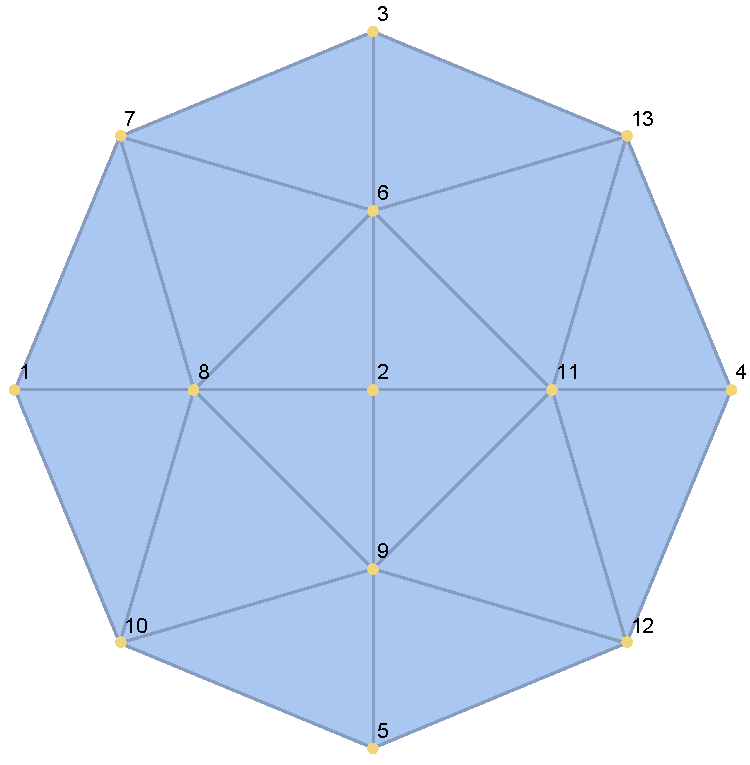
\includegraphics[width=\linewidth]{img/typicalMesh.pdf}
	\caption{Типичная триангуляция диска}\label{fig:typicalMesh}
	\endminipage\hfill
	\minipage{0.45\textwidth}
	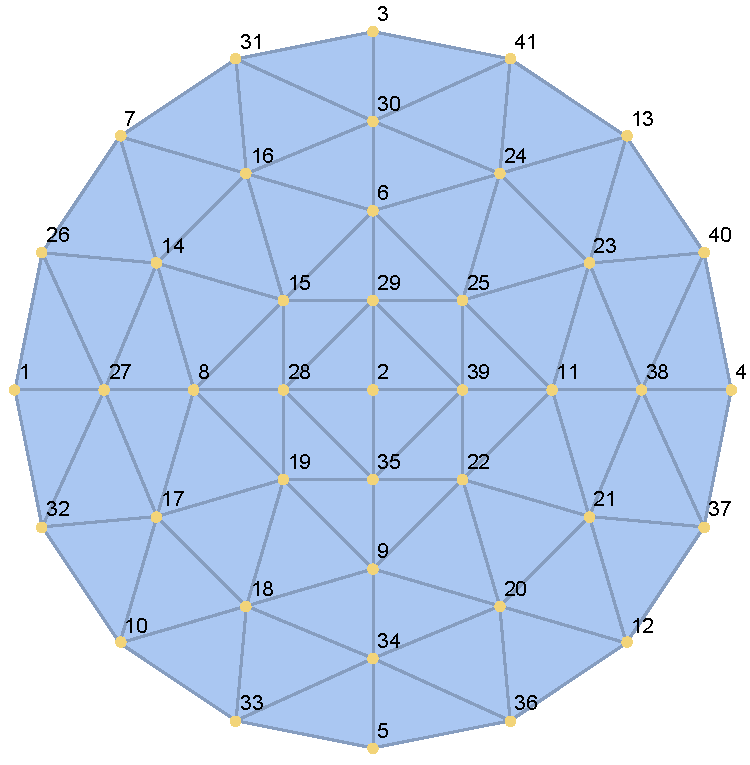
\includegraphics[width=\linewidth]{img/typicalMeshRefined.pdf}
	\caption{Измельчённая триангуляция диска. Обратите внимание, что кривизна границы с измельчением учитывается}\label{fig:typicalMeshRefined}
	\endminipage
\end{figure}

\begin{figure}[!h]
	\centering
	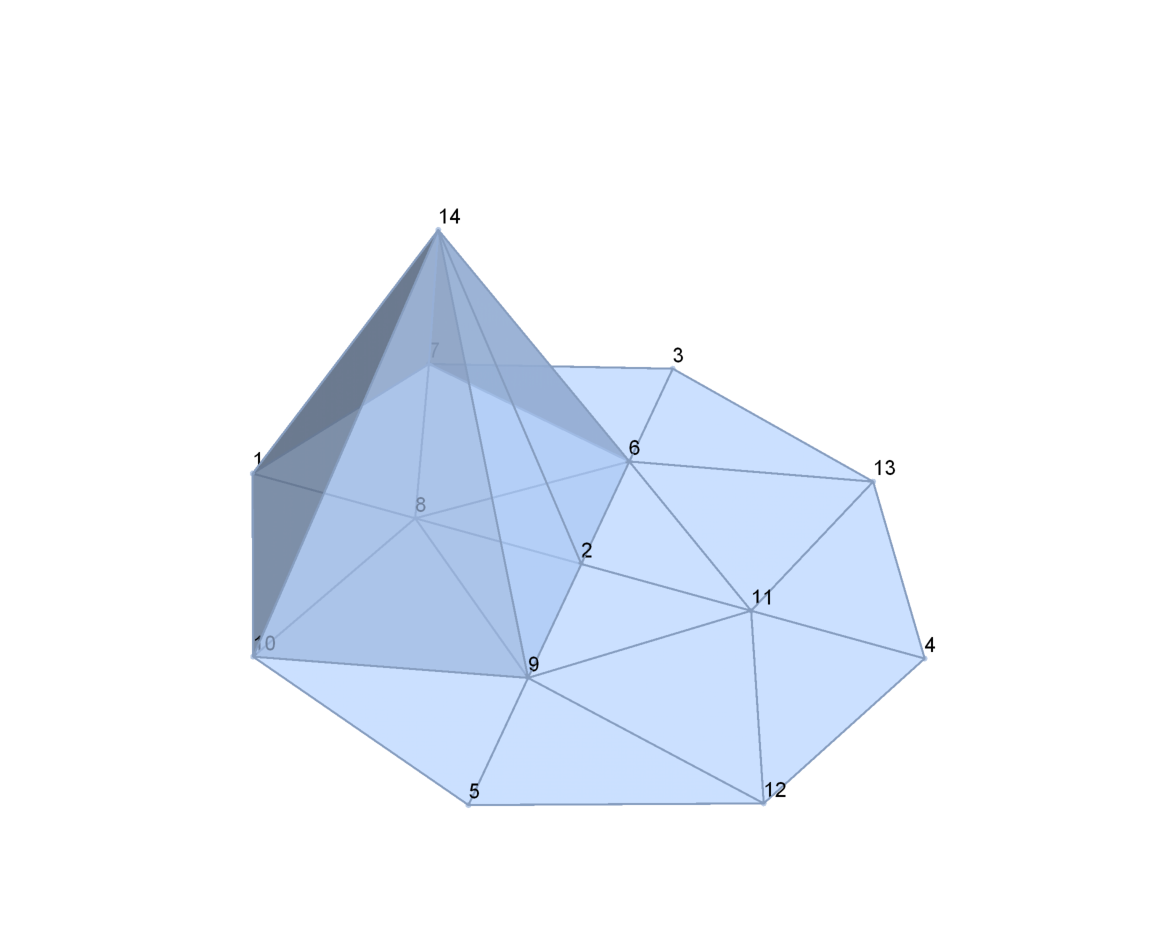
\includegraphics[width=0.8\linewidth]{img/typicalBasisFunc.pdf}
	\caption{Базисная функция $\phi_8$, определённая на сетке рис.~\ref{fig:typicalMesh}}
	\label{fig:typicalBasisFunc}
\end{figure}

Пусть $\Omega_h$ есть триангуляция области $\Omega$ --- множество вершин и элементов (треугольников). При этом каждый треугольник даёт в пересечении с другим треугольником либо пустое множество, либо вершину, либо ребро --- иными словами, триангуляция не может иметь «висячих» вершин. Очевидным требованием является сходимость меры $\Omega_{h / k}$ к мере $\Omega$ при $k \rightarrow \infty$. \\
Для триангуляций, вообще говоря, придумано целое множество абстракций для представления в компьютере. Более подробно мы обсудим этот вопрос позже, когда станут ясны все требования к нашей сетке.

Возьмём в качестве пространства $\mathbb{V}_h$ пространство всех непрерывных и линейных на каждом треугольнике функций, определённых на $\Omega_h$:
\begin{align}
	\mathbb{V}_h &= C^0(\Omega) \cap \{ v : v|_\Delta \in P_1(\Delta) \text{ для всех треугольников } \Delta \in \Omega_h \}, \label{Vh} \\
	P_1(\Delta) & \coloneqq \{ v : v(x, \, y) = c_1 \, x + c_2 \, y + c_3, \: (x, \, y) \in \Delta \} \label{p1Space}
\end{align}

В качестве базиса $\mathbb{V}_h$ выберем \textit{вершинный} базис (см. рис.~\ref{fig:typicalBasisFunc}):
\begin{align}
	\label{nodalBasis}
	\phi_i(\vect{x}_j) = \delta_{i \, j} \text{ для всех вершин } \vect{x_j} \text{ триангуляции } \Omega_h,
\end{align}
т.\,е. $i$--я функция базиса принимает единицу в $i$--й вершине и ноль иначе. 

В таком выборе базиса есть, как минимум, четыре преимущества:
\begin{enumerate}
	\item простота интерпретации базисных коэффициентов --- $u_h(\vect{x}_i) = \xi_i$,
	\item (вытекает из первого пункта) простота построения интерполяции $\pi_1 g(\vect{x}) \coloneqq \sum_1^n g(\vect{x}_i) \, \phi_i(\vect{x})$ любой известной функции $g$. Это полезно для расчёта квадратур, входящих в систему~(\ref{SLAE}),
	\item финитность базисных функций и, как следствие, \textbf{разреженность матрицы $\vect{A}$} и 
	\item элегантность алгоритма ассемблирования системы~(\ref{SLAE}) (подробно рассмотрим в разделе~(\ref{assembly})).
\end{enumerate} 

Третий пункт особенно важен, так как он позволяет решать задачи, приводящие к огромным СЛАУ, пользуясь ограниченной памятью компьютера.

\subsection{Учёт краевых условий}

Задание граничных условий~(\ref{BCs}) в виде тройки функций~$(\kappa, \, g_D, \, g_N)$ удобно тем, что оно единообразно описывает все три классических типа краевых условий: Дирихле, Неймана и Робина.

Пусть $\Gamma_D$, $\Gamma_N$ и $\Gamma_R \subset \partial \Omega$ суть не пересекающиеся части границы, в объединении дающие $\partial \Omega$, на которых заданы краевые условия Дирихле, Неймана и Робина соответственно. Задания условий на поток через границу очевидны; для условий Неймана достаточно положить $\kappa(\Gamma_N) = \{ 0 \}$, для условий Робина --- $g_D(\Gamma_R) = \{ 0 \}$:
\begin{align*}
\vect{\hat{n}} \cdot (a \, \nabla u) = g_N,               &\quad \vect{x} \in \Gamma_N, \\
\vect{\hat{n}} \cdot (a \, \nabla u) + \kappa \, u = g_N, &\quad \vect{x} \in \Gamma_R.
\end{align*}

Краевые условия Дирихле $u = g_D, \: \vect{x} \in \Gamma_D$ нельзя учесть явно с использованием~(\ref{BCs}), однако их можно аппроксимировать условиями Робина. Перепишем~(\ref{BCs}) в виде
$$
u - g_D = \frac{ g_N - \vect{\hat{n}} \cdot (a \, \nabla u) }{ \kappa }.
$$

Положив $g_N(\Gamma_D) = \{ 0 \}$ и $\kappa(\Gamma_D)$ достаточно большим (скажем, порядка $10^{50}$), получим $u - g_D \simeq 0$ --- фактически равенство в конечной арифметике компьютера.

С практической точки зрения такой учёт условий Дирихле означает внесение возмущений в $\vect{A}$ и $\vect{b}$ --- взгляните на элементы матрицы и вектора Робина~(\ref{RobinMatrixEl}) и~(\ref{RobinVectorEl}). \\
В них дают вклад интегралы, в интегранды которых входит $\kappa = 10^{50}$. 

Существует два распространённых способа учёта условий Дирихле:
\begin{enumerate}
	\item для всех $\vect{x}_j \in \Gamma_D$ обнулить $j$--ю строчку матрицы~$\vect{A}$, установить $\vect{A}_{j \, j} = 1$ и $\vect{b}_{j} = g_D(\vect{x}_j)$,
	\item для всех $\vect{x}_j \in \Gamma_D$ положить $\vect{b}_{j} = g_D(\vect{x}_j)$ и домножить $\vect{b}_{j}$ и $\vect{A}_{j \, j}$ на большое число (скажем, на $10^{50}$).
\end{enumerate}

Первый подход фактически заменяет $j$--е уравнение системы~(\ref{SLAE}) на уравнение $\xi_j =  g_D(\vect{x}_j)$, второй --- на уравнение $\xi_j \simeq g_D(\vect{x}_j)$, нивелируя вклад остальных слагаемых уравнения\footnote{
	В МКЭ в качестве базиса выбирают \textit{вершинный базис}, т.\,е. такой, что $\phi_i(\vect{x}_j) = \delta_{i \, j}$ (символ Кронекера). Поэтому вес $\xi_j$ суть значение функции $u_h$ в $j$--м узле. 	
}.

По своей сути наш подход совпадает со вторым, однако у него есть приятный бонус: нет никакой необходимости заботиться об учёте условий Дирихле отдельно, изменяя матрицу и вектор системы --- \textit{учёт условий всех типов происходит единообразно}.

Первый подход наиболее «честный» в том смысле, что решение ищется в «правильном» пространстве $\mathbb{V}_{h, \, D} := \mathbb{V}_h \cap \{ v : v(\vect{x}) = g_D(\vect{x}) \text{ для всех } \vect{x} \in \Gamma_{D} \}$. Однако такой подход нарушает симметричность матрицы $\vect{A}$. Как следствие, приходится либо симметризовывать матрицу, либо использовать несимметричный формат хранения, увеличивая расходы на память компьютера.

В данной работе мы не будем использовать первый подход.

\subsection{Ассемблирование СЛАУ}
\label{assembly}

\subsubsection{Вклады квадратур по элементам}
\label{elementAssembly}

В сердце МК\textbf{Э} --- ассемблирование матрицы~\vect{A} и вектора~\vect{b}, которое очень удобно и быстро осуществлять при обходе \textbf{элементов} (в нашем случае --- треугольников) сетки $\Omega_h$. Отсюда первое требование к абстракции для сетки --- \textbf{элементы необходимо хранить явно}.

Рассмотрим процесс сборки на примере $\Omega_h$, представленной на рис.~\ref{fig:assemblyMesh}.

\begin{figure}[!h]
	\centering
	\resizebox{0.8\textwidth}{!}{\input{img/assemblyMesh.pdf_tex}}
	\caption{{\color{Plum} Глобальная нумерация узлов}, {\color{OliveGreen} локальная нумерация узлов} и глобальная нумерация элементов, задаваемые абстракциями $\vect{\mathcal{V}}$ и $\vect{\mathcal{T}}$}
	\label{fig:assemblyMesh}
\end{figure}

Триангуляция\footnote{
	Здесь и далее для упрощения нотаций мы будем использовать верхний индекс со скобками $(i)$ для указания того, что объект имеет отношение к $i$--му элементу сетки $\Delta^{(i)}$.
} $\Omega_h = \cup_1^3 \Delta^{(i)}$ (рис.~\ref{fig:assemblyMesh}) может быть представлена списком вершин $\vect{\mathcal{V}}$ и «треугольников» (указатели на элементы $\vect{\mathcal{V}}$) $\vect{\mathcal{T}}$:
\begin{align*}
	\vect{\mathcal{V}} &\coloneqq \langle \quad
		( \frac{1}{2}, \, \frac{\sqrt{2}}{2} ), \,
		( -\frac{1}{2}, \, \frac{\sqrt{2}}{2} ), \,
		( \frac{3}{2}, \, \frac{\sqrt{2}}{2} ), \,
		(1, \, 0), \,
		(0, \, 0)
	\quad \rangle, \\
	\vect{\mathcal{T}} &\coloneqq \langle \quad
	( 5, \, 4, \, 1 ), \,
	( 1, \, 4, \, 3 ), \,
	( 2, \, 5, \, 1 )
	\quad \rangle.
\end{align*}

Заметим, что каждый элемент $\vect{\mathcal{T}}_i$ определяет отображение $\vect{\mathcal{n}}^{(i)} \: : \: \{ 1, \, 2, \, 3 \} \rightarrow \{ \vect{\mathcal{T}}_{i \, 1}, \, \vect{\mathcal{T}}_{i \, 2}, \, \vect{\mathcal{T}}_{i \, 3} \}$ {\color{OliveGreen} локальной} нумерации вершин на {\color{Plum} глобальную}. \\
Например, для первого треугольника $\Delta^{(1)}$ соответствие между {\color{OliveGreen} локальной} и {\color{Plum} глобальную} нумерацией определяется $\vect{\mathcal{n}}^{(1)}({\color{OliveGreen} 1}) = {\color{Plum} 5}$, $\vect{\mathcal{n}}^{(1)}({\color{OliveGreen} 2}) = {\color{Plum} 4}$ и $\vect{\mathcal{n}}^{(1)}({\color{OliveGreen} 3}) = {\color{Plum} 1}$ (см. рис.~\ref{fig:assemblyMesh}).

Вершины $\vect{x}^{(i)}_1 \coloneqq (x^{(i)}_1, \, y^{(i)}_1)$, $\vect{x}^{(i)}_2 \coloneqq (x^{(i)}_2, \, y^{(i)}_2)$ и $\vect{x}^{(i)}_3 \coloneqq (x^{(i)}_3, \, y^{(i)}_3)$, образующие треугольник $\Delta^{(i)}$, могут быть получены так:
$$
	\vect{x}^{(i)}_j = \vect{\mathcal{V}}_{\mathcal{n}_i(j)}.
$$
Продемонстрируем ассемблирование на примере матрицы масс:
\begin{align}
\label{massMatrixAssembly}
	\begin{split}
		\vect{M} =
		& 
		\int_{\Omega_h} c 
			\begin{bmatrix}
				\phi_1 \, \phi_1 & \phi_1 \, \phi_2 & \phi_1 \, \phi_3 & \phi_1 \, \phi_4 & \phi_1 \, \phi_5 \\
				                 & \phi_2 \, \phi_2 & \phi_2 \, \phi_3 & \phi_2 \, \phi_4 & \phi_2 \, \phi_5 \\
				                 &                  & \phi_3 \, \phi_3 & \phi_3 \, \phi_4 & \phi_3 \, \phi_5 \\
				                 &                  &                  & \phi_4 \, \phi_4 & \phi_4 \, \phi_5 \\	
				\text{сим.}	     &                  &                  &                  & \phi_5 \, \phi_5			               
			\end{bmatrix}
		\diff{\vect{x}} 
		= \\
		&
		\int_{\Delta_1} c 
		\begin{bmatrix}
			\phi_1 \, \phi_1 & 0 & 0 & \phi_1 \, \phi_4 & \phi_1 \, \phi_5 \\
			&0&0&0&0 \\
			&&0&0&0 \\
			&&& \phi_4 \, \phi_4 & \phi_4 \, \phi_5 \\	
			\text{сим.}	&&&& \phi_5 \, \phi_5			               
		\end{bmatrix}
		\diff{\vect{x}} 
		+
		\int_{\Delta_2} c 
		\begin{bmatrix}
			\phi_1 \, \phi_1 & 0 & \phi_1 \, \phi_3 & \phi_1 \, \phi_4 & 0 \\
			&0&0&0&0 \\
			&& \phi_3 \, \phi_3 & \phi_3 \, \phi_4 & 0 \\
			&&& \phi_4 \, \phi_4 & 0 \\	
			\text{сим.} &&&& 0			               
		\end{bmatrix}
		\diff{\vect{x}}
		+ \\
		&
		\int_{\Delta_3} c 
		\begin{bmatrix}
			\phi_1 \, \phi_1 & \phi_1 \, \phi_2 & 0 & 0 & \phi_1 \, \phi_5 \\
			& \phi_2 \, \phi_2 & 0 & 0 & \phi_2 \, \phi_5 \\
			&&0&0&0 \\
			&&&0&0 \\
			\text{сим.} &&&& \phi_5 \, \phi_5			               
		\end{bmatrix}
		\diff{\vect{x}}
	\end{split}
\end{align}
В~(\ref{massMatrixAssembly}) мы воспользовались аддитивностью интеграла и финитностью базисных функций --- из построения базиса очевидно, что вклад в матрицу на треугольнике $\Delta^{(i)}$ дадут лишь три базисные функции, принимающие единицу в образующих его узлах (cм. рис.~\ref{fig:localBasis}).

На практике на каждом элементе $\Delta^{(i)}$ считается \textbf{локальная матрица} размерности $3 \times 3$
\begin{equation}
\label{localMassMatrix}
	\vect{\hat{M}}^{(i)} 
	=
	\int_{\Delta^{(i)}} c 
	\begin{bmatrix}
		\hat{\phi}^{(i)}_1 \, \hat{\phi}^{(i)}_1 & \hat{\phi}^{(i)}_1 \, \hat{\phi}^{(i)}_2 & \hat{\phi}^{(i)}_1 \, \hat{\phi}^{(i)}_3 \\
		& \hat{\phi}^{(i)}_2 \, \hat{\phi}^{(i)}_2 & \hat{\phi}^{(i)}_2 \, \hat{\phi}^{(i)}_3 \\
		\text{cим.} && \hat{\phi}^{(i)}_3 \, \hat{\phi}^{(i)}_3		               
	\end{bmatrix}
	\diff{\vect{x}},
\end{equation}
где $\hat{\phi}^{(i)}_j \coloneqq \phi_{\vect{\mathcal{n}}^{(i)}(j)}|_{\Delta^{(i)}}$ --- \textbf{локальная базисная функция} (см. рис.~\ref{fig:localBasis}); затем вносится вклад в матрицу системы $\vect{A}_{ \vect{\mathcal{n}}^{(i)}(j) \, \vect{\mathcal{n}}^{(i)}(k) } = \vect{A}_{ \vect{\mathcal{n}}^{(i)}(j) \, \vect{\mathcal{n}}^{(i)}(k) } + \vect{\hat{M}}_{j \, k}, \quad j = 1, \, 2, \, 3, \quad k = j, \, \dots, \, 3$ и осуществляется переход к следующему элементу $\Delta_{i+1}$.

Формулы для локальных базисных функций легко получить из определения~(\ref{nodalBasis}), записанного в матричном виде. $\hat{\phi}^{(i)}_j(x, \, y) = c^{(i)}_{j\,1} \, x + c^{(i)}_{j\,2} \, y + c^{(i)}_{j\,3}$ и 
\begin{equation}
\label{basisCoef}
	\underbrace{
		\begin{bmatrix}
			c^{(i)}_{1\,1} & c^{(i)}_{1\,2} & c^{(i)}_{1\,3} \\
			c^{(i)}_{2\,1} & c^{(i)}_{2\,2} & c^{(i)}_{2\,3} \\
			c^{(i)}_{3\,1} & c^{(i)}_{3\,2} & c^{(i)}_{3\,3}               
		\end{bmatrix}
	}_{\eqqcolon \vect{C}^{(i)}}
	\begin{bmatrix}
		x^{(i)}_1 & x^{(i)}_2 & x^{(i)}_3 \\
		y^{(i)}_1 & y^{(i)}_2 & y^{(i)}_3 \\
		1 & 1 & 1               
	\end{bmatrix}
	=
	\begin{bmatrix}
		1 & 0 & 0 \\
		0 & 1 & 0 \\
		0 & 0 & 1               
	\end{bmatrix},
\end{equation}
поэтому $\hat{\phi}^{(i)}_j = (\vect{C}^{(i)})^{-1}_{\cdot \, j} \cdot (x, \, y, \, 1)$.

Коэффициент реакции $c(\vect{x})$ может быть, вообще говоря, произвольной функцией. Поэтому для расчёта квадратур в~(\ref{localMassMatrix}) удобно заменить его линейной (или квадратичной) интерполяцией
\begin{subequations}
\label{interpolation}
	\begin{align}
		c|_{\Delta^{(i)}} \simeq 
		\pi_1 c^{(i)}(\vect{x}) & \coloneqq \sum_{j=1}^3 c(\vect{x}^{(i)}_j) \, \hat{\phi}^{(i)}_j(\vect{x}) \text{ или } \\
		\pi_2 c^{(i)}(\vect{x}) & \coloneqq \sum_{j=1}^6 c(\vect{x}^{(i)}_j) \, \hat{\psi}^{(i)}_j(\vect{x})
	\end{align}
\end{subequations}
где $\hat{\psi}^{(i)}_1$, $\hat{\psi}^{(i)}_2$, \dots, $\hat{\psi}^{(i)}_6$ --- квадратичные базисные функции (см. рис.~\ref{fig:localQuadBasis}), принимающие единицы на вершинах треугольника $\Delta^{(i)}$ и серединах его рёбер 
\begin{equation}
	\vect{x}^{(i)}_4 \coloneqq \frac{\vect{x}^{(i)}_2 + \vect{x}^{(i)}_3}{2},
	\quad
	\vect{x}^{(i)}_5 \coloneqq \frac{\vect{x}^{(i)}_1 + \vect{x}^{(i)}_3}{2},
	\quad
	\vect{x}^{(i)}_6 \coloneqq \frac{\vect{x}^{(i)}_1 + \vect{x}^{(i)}_2}{2}.
\end{equation}
Формулы для квадратичного базиса могут быть получены аналогично~(\ref{basisCoef}). Более того, можно заметить, что локальные квадратичные базисные функции можно выразить через произведения локальных линейных базисных функций.

Очевидно, что 	
\begin{align}
	c|_{\Delta^{(i)}} &= \pi_1 c^{(i)}(\vect{x}), \text{ если } c|_{\Delta^{(i)}} \in P_1(\Delta^{(i)}), \\
	c|_{\Delta^{(i)}} &= \pi_2 c^{(i)}(\vect{x}), \text{ если } c|_{\Delta^{(i)}} \in P_2(\Delta^{(i)}),
\end{align}
где $P_2(\Delta^{(i)})$ (аналогично $P_1(\Delta^{(i)})$, определённое в~(\ref{p1Space})) есть пространство полиномов 2-й степени, определённых на $i$--м элементе: 
\begin{align}
	P_2(\Delta^{(i)}) & \coloneqq \{ v : v(x, \, y) = c_1 \, x^2 + c_2 \, y^2 + c_3 \, x \, y + c_4 \, x + c_5 \, y + c_6, \: (x, \, y) \in \Delta^{(i)} \}, \\
	P_1(\Delta^{(i)}) & \subset P_2(\Delta^{(i)}).
\end{align}
Если же $c(\vect{x})$ не является полиномом, то с дроблением сетки интерполяция~(\ref{interpolation}) будет всё лучше его аппроксимировать.

\begin{figure}[!h]
	\minipage{0.45\textwidth}
	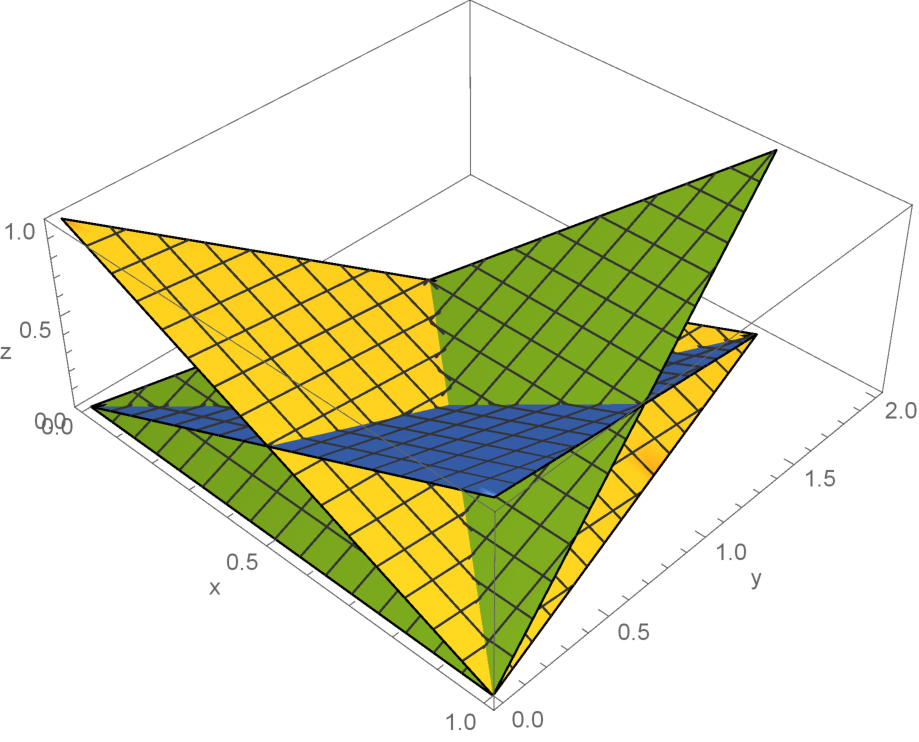
\includegraphics[width=\linewidth]{img/localBasis.pdf}
	\caption{Локальные базисные функции $\hat{\phi}^{(i)}_1$, $\hat{\phi}^{(i)}_2$ и $\hat{\phi}^{(i)}_3$, линейные на $i$-м элементе}\label{fig:localBasis}
	\endminipage\hfill
	\minipage{0.45\textwidth}
	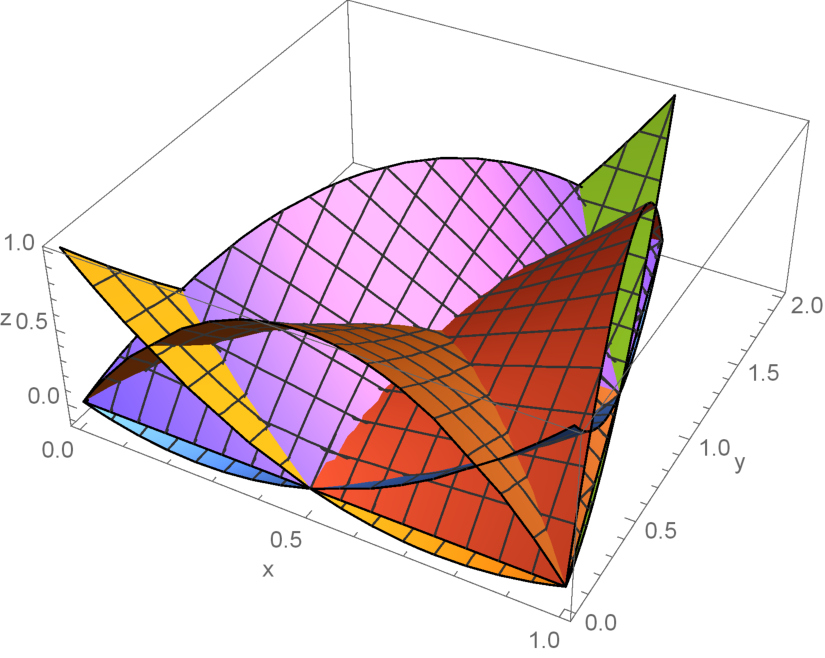
\includegraphics[width=\linewidth]{img/localQuadBasis.pdf}
	\caption{Локальные базисные функции $\hat{\psi}^{(i)}_1$, $\hat{\psi}^{(i)}_2$, \dots, $\hat{\psi}^{(i)}_6$, квадратичные на $i$-м элементе}\label{fig:localQuadBasis}
	\endminipage
\end{figure}

С учётом интерполяции~(\ref{interpolation}) и сказанного выше, вычисление квадратур для~(\ref{localMassMatrix}) сводится к вычислению интегралов типа
\begin{equation}
	\int_{\Delta^{(i)}} (\hat{\phi}^{(i)}_1(\vect{x}))^m \, (\hat{\phi}^{(i)}_2(\vect{x}))^l \, (\hat{\phi}^{(i)}_3(\vect{x}))^k \diff{\vect{x}},
\end{equation} 
вид которых известен (или может быть быстро посчитан, например, в системе \texttt{Mathematica}).

Сборка матрицы $\vect{S}$ и вектора $\vect{f}$ абсолютно аналогична, поэтому выкладки мы приводить не будем. \\
В секции~(\ref{localMatricesAndVectors}) приведены формулы для расчёта всех локальных матриц и векторов~(\ref{how2compute}), необходимых для сборки системы.

\subsubsection{Вклады квадратур по границе}
\label{boundaryAssembly}

Для того, чтобы ассемблировать вклады матрицы и вектора Робина, необходимо иметь доступ к границе $\Omega_h$. \textbf{Это второе требование к абстракции для нашей триангуляции}.

В принципе, можно было бы хранить список граничных «рёбер» --- список пар указателей на вершины в списке $\vect{\mathcal{V}}$ (подобно тому, как мы поступили с абстракцией для элементов $\vect{\mathcal{T}}$). \\
Однако мы откажемся от такого подхода по причинам, изложенным ниже.

\paragraph{Измельчение сетки и связанные с этим требования к абстракции для триангуляции}

Для уточнения решения часто необходимо измельчить сетку $\Omega_h$ --- решить задачу на более точной триангуляции $\Omega_\frac{h}{2}$. При этом дробиться могут не обязательно все\footnote{
	Примером может служить \textbf{адаптивный МКЭ} (\textit{adaptive FEM}). По окончании решения используется апостериорная оценка ошибки (основанная на скачках в градиентах полученного решения $u_h$), на основании которой конечное количество треугольников измельчается и решение пересчитывается.\\
	Об адаптивном МКЭ можно прочесть в~\cite[c.~97]{umea}.
} элементы $\Delta^{(i)}$.

Поэтому третье требование к абстракции --- возможность измельчать исходную сетку $\Omega_h$.

Добавление элементов (а значит, и новых узлов) приводит к появлению «висячих» вершин (мы обсудили это в секции~\ref{workOnDiscreteMesh}), нарушающих структуру триангуляции.

Чтобы избежать этой проблемы, удобно иметь доступ к $0 \le k \le 3$ смежным треугольникам («соседям») $\Delta^{(j)}$ текущего треугольника $\Delta^{(i)}$.\\ Для этого введём новую абстракцию $\vect{\mathcal{N}}$, элемент $\vect{\mathcal{N}}_i$ которой содержит тройку указателей на элементы $\vect{\mathcal{T}}$, являющиеся соседями элемента $\Delta^{(i)}$, описываемого $i$--м элементом абстракции $\vect{\mathcal{T}}$. Для сетки рис.~\ref{fig:assemblyMesh} описанная структура будет иметь вид:
\begin{subequations}
	\label{nodesAndNeighbors}
	\begin{align}
		\vect{\mathcal{V}} &\coloneqq \langle \quad
		( \frac{1}{2}, \, \frac{\sqrt{2}}{2} ), \,
		( -\frac{1}{2}, \, \frac{\sqrt{2}}{2} ), \,
		( \frac{3}{2}, \, \frac{\sqrt{2}}{2} ), \,
		(1, \, 0), \,
		(0, \, 0)
		\quad \rangle, \\
		\vect{\mathcal{T}} &\coloneqq \langle \quad
		( 5, \, 4, \, 1 ), \,
		( 1, \, 4, \, 3 ), \,
		( 2, \, 5, \, 1 )
		\quad \rangle, \\
		\vect{\mathcal{N}} &\coloneqq \langle \quad
		( 2, \, 3, \, -1 ), \,
		( -1, \, -1, \, 1 ), \,
		( 1, \, -1, \, -1 )
		\quad \rangle.
	\end{align}
\end{subequations}

Обратите внимание, что если ребро треугольника $\vect{\mathcal{T}}_i$ напротив $k$--го узла $\vect{\mathcal{V}}_{\vect{\mathcal{n}}_i(k)}$ является частью границы (т.\,е. у треугольника нет соседа по этому ребру), то $\vect{\mathcal{N}}_{i\,k} = -1$. \\
Например, как видно из рис.~\ref{fig:assemblyMesh} и~(\ref{nodesAndNeighbors}), 3--е ребро (ребро напротив 3--й вершины) 1--го треугольника является частью границы. Поэтому $\vect{\mathcal{N}}_{1\,3} = -1$.

Условимся, что узлы в тройках $\vect{\mathcal{T}}_{i}$ занумерованы так, что обход вершин $i$-го треугольника ведётся \textbf{против часовой стрелки} (справедливо для нашего примера~(\ref{nodesAndNeighbors})). Это удобно, потому что интегралы по границе в~(\ref{multByTestFunc}) берутся при её обходе против часовой стрелки.\\
Таким образом, не будет путаницы при учёте знака в процессе сборки вкладов матрицы~(\ref{RobinMatrixEl}) и вектора Робина~(\ref{RobinVectorEl}) в СЛАУ~(\ref{SLAE}).

Структура $\langle \vect{\mathcal{V}}, \, \vect{\mathcal{T}}, \, \vect{\mathcal{N}}\rangle$ называется «\textbf{узлы и треугольники}» (см.~\cite[с.~14]{delaunay}).

При использовании данной структуры все перечисленные выше требования к абстракции для триангуляции выполняются. Как было замечено в начале раздела~\ref{boundaryAssembly}, мы освобождены от необходимости явного хранения границы --- мы можем легко получить её при обходе элементов $\Delta^{(i)}$: если $\vect{\mathcal{N}}_{i\,k} < 0$, то ребро $(\vect{\mathcal{V}}_{\vect{\mathcal{n}}_i(k \dotplus 1)}, \, \vect{\mathcal{V}}_{\vect{\mathcal{n}}_i(k \dotplus 2)})$ суть часть $\partial \Omega$. Здесь через «$\dotplus$» обозначено сложение по модулю 4: $2 \dotplus 1 = 3$, $2 \dotplus 2 = 1$ и т.\,д.

Вывод формул для локальных матрицы и вектора Робина мы не будем приводить здесь, потому что он аналогичен выводу локальной матрицы масс $\vect{\hat{M}}^{(i)}$, приведённому в разделе~\ref{elementAssembly}. Как видно из рис.~\ref{fig:localBasis}, лишь две локальные базисные функции дают вклад в интеграл по ребру, поэтому размерности $\vect{\hat{R}}^{(i)}$ и $\vect{\hat{r}}^{(i)}$ --- 2 $\times$ 2 и 2 соответственно.

В секции~(\ref{localMatricesAndVectors}) приведены формулы для расчёта всех локальных матриц и векторов~(\ref{how2compute}), необходимых для сборки системы.

\newpage
\vfill
\begin{landscape}
	\subsubsection{Формулы для локальных матриц и векторов}
	\label{localMatricesAndVectors}
	
	Для упрощения нотаций в таблице~\ref{tab:localMatricesAndVectorsFormulas} мы не стали указывать индекс элемента ($\Delta$ вместо $\Delta^{(i)}$, $\vect{\hat{M}}$ --- вместо $\vect{\hat{M}}^{(i)}$ и т.\,д.). Через $\Delta$, как всегда, обозначен элемент, через $e$ --- граничное ребро.
	
	В матрицах (векторах) с интегралами по элементам через $(x_1, y_1)$, $(x_2, y_2)$ и $(x_3, y_3)$ обозначены образующие элемент вершины; в матрице и векторе Робина через  $(x_1, y_1)$ и $(x_2, y_2)$ обозначены вершины, образующие ребро.  
	
	Для краткости образ точки $(x_j, y_j)$ мы обозначили $f_j \coloneqq f(x_j, y_j)$, $\kappa_j \coloneqq \kappa(x_j, y_j)$ и т.\,д.
	
	\begin{table}[h]
		\caption{Формулы для локальных матриц (векторов), необходимые для сборки вкладов от~(\ref{how2compute}) в СЛАУ~(\ref{SLAE})}
		\label{tab:localMatricesAndVectorsFormulas}
		\begin{center}\begin{tabular}{ccrl}
				\toprule
				\multicolumn{2}{c}{\textbf{Локальная матрица (вектор)}} & \multicolumn{2}{c}{\textbf{Формула}}\\
				\midrule
				$\vect{\hat{M}}$
				&
				$c \in P_1$
				&
				$\frac{\area \Delta}{60}$
				&
				$\begin{pmatrix*}[l]
					6 \, c_1 + 2 \, c_2 + 2 \, c_3 & 
					2 \, c_1 + 2 \, c_2 + c_3 & 
					2 \, c_1 + c_2 + 2 \, c_3 \\
					& 2 \, c_1 + 6 \, c_2 + 2 \, c_3 & 
					c_1 + 2 \, c_2 + 2 \, c_3 \\
					\text{сим.}	&& 2 \, c_1 + 2 \, c_2 + 6 \, c_3 		               
				\end{pmatrix*}$ \\
				\midrule
				$\vect{\hat{S}}$ 
				&
				$a \in P_1$ 
				& 
				$\frac{a_1 + a_2 + a_3}{12 \area \Delta}$
				&
				$\begin{pmatrix*}[l]
					(x_2 - x_3)^2 + (y_2 - y_3)^2 & 
					(x_1 - x_3) (x_3 - x_2) + (y_1 - y_3) (y_3 - y_2) & 
					(x_1 - x_2) (x_2 - x_3) + (y_1 - y_2) (y_2 - y_3) \\
					& (x_1 - x_3)^2 + (y_1 - y_3)^2 & 
					(x_2 - x_1) (x_1 - x_3) + (y_2 - y_1) (y_1 - y_3) \\
					\text{сим.}	&& (x_1 - x_2)^2 + (y_1 - y_2)^2            
				\end{pmatrix*}$ \\
				\midrule
				$\vect{\hat{S}}$ 
				&
				$a \in P_2$ 
				& 
				$\frac{a_3 + a_4 + a_5}{12 \area \Delta}$
				&
				$\begin{pmatrix*}[l]
					(x_2 - x_3)^2 + (y_2 - y_3)^2 & 
					(x_1 - x_3) (x_3 - x_2) + (y_1 - y_3) (y_3 - y_2) & 
					(x_1 - x_2) (x_2 - x_3) + (y_1 - y_2) (y_2 - y_3) \\
					& (x_1 - x_3)^2 + (y_1 - y_3)^2 & 
					(x_2 - x_1) (x_1 - x_3) + (y_2 - y_1) (y_1 - y_3) \\
					\text{сим.}	&& (x_1 - x_2)^2 + (y_1 - y_2)^2            
					\end{pmatrix*}$ \\
				\midrule
				$\vect{\hat{R}}$ 
				&
				$\kappa \in P_1$ 
				& 
				$\frac{\length e}{12}$
				&
				$\begin{pmatrix*}[l]
					3 \, \kappa_1 + \kappa_2 & \kappa_1 + \kappa_2 \\
					\text{сим.}	& \kappa_1 + 3 \, \kappa_2            
				\end{pmatrix*}$ \\
				\midrule
				$\vect{\hat{f}}$
				&
				$f \in P_1$ 
				& 
				$\frac{\area \Delta}{12}$
				&
				$\begin{pmatrix*}[l]
					2 \, f_1 + f_2 + f_3 \\
					f_1 + 2 \, f_2 + f_3 \\
					f_1 + f_2 + 2 \, f_3          
				\end{pmatrix*}$ \\
				\midrule
				$\vect{\hat{f}}$
				&
				$f \in P_2$ 
				& 
				$\frac{\area \Delta}{60}$
				&
				$\begin{pmatrix*}[l]
					2 f_1 - f_2 - f_3 + 4 f_4 +8 f_5 + 8 f_6 \\
					f_1-2 f_2+f_3-4 \left(2 f_4+f_5+2 f_6\right) \\
					f_1+f_2-2 \left(f_3+4 \left(f_4+f_5\right)+2 f_6\right)        
				\end{pmatrix*}$ \\
				\midrule
				$\vect{\hat{r}}$
				&
				$\kappa, \, g_D, \, g_N \in P_1$ 
				&
				$\frac{\length e}{12}$
				&
				$\begin{pmatrix*}[l]
					\left(\kappa _1+\kappa _2\right) g_{D_2}+\left(3 \kappa _1+\kappa _2\right) g_{D_1}+4 g_{N_1}+2 g_{N_2} \\
					\left(\kappa _1+\kappa _2\right) g_{D_1}+\left(\kappa _1+3 \kappa _2\right) g_{D_2}+2 g_{N_1}+4 g_{N_2}        
				\end{pmatrix*}$ \\
				\bottomrule
			\end{tabular}\end{center}
	\end{table}
\end{landscape}
\vfill
\newpage

\subsection{Генерация портрета матрицы, абстракция для матрицы и решение системы}
Мы уже упомянули тот факт, что матрица системы есть \textbf{разреженная} матрица. Портрет матрицы тесно связан с видом триангуляции: его легко определить, имея список смежных вершин к данной вершине --- произведение базисных функций $\phi_i(\vect{x}) \, \phi_j(\vect{x})$, как видно из их определения, даст не ноль только тогда, когда $\vect{x}_i$ и $\vect{x}_j$ связаны ребром.

Используемый формат для абстракции разреженной матрицы --- \textbf{симметричный CSlR--формат} (\textit{compressed sparse (lower triangular) row}), который иногда называют \textbf{симметричным разреженно--строчным форматом}.\\
О данном формате можно прочесть в~\cite[с.~5]{sparskit}.

\begin{figure}[!hb]
	\minipage{0.4\textwidth}
	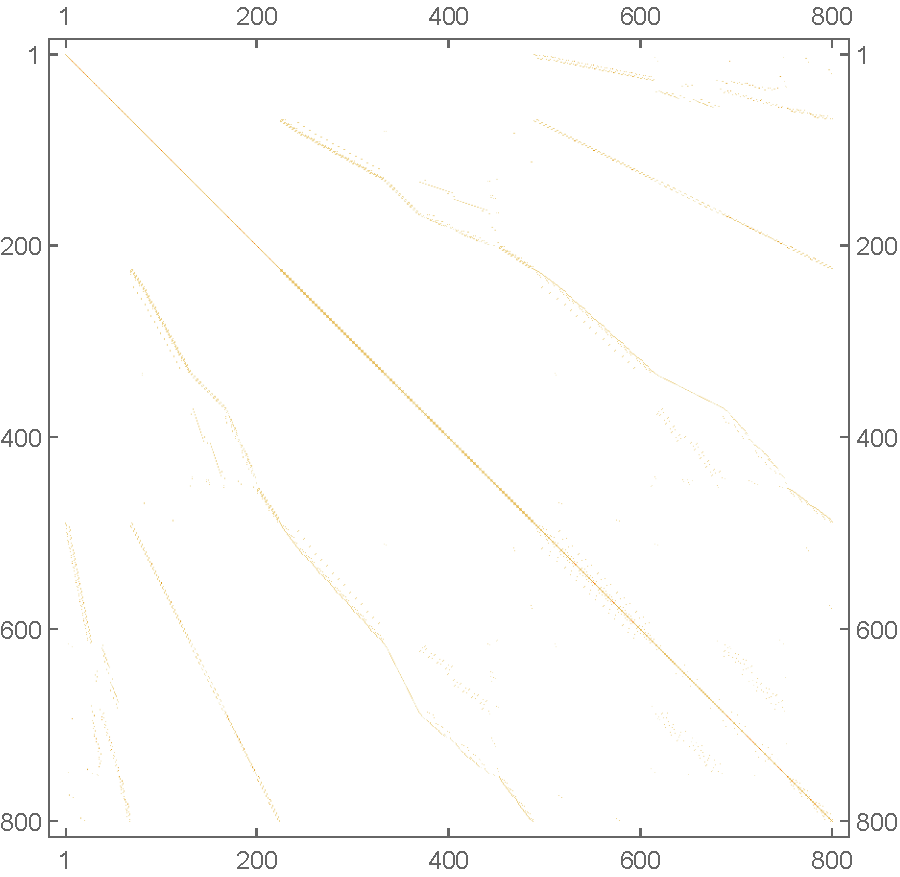
\includegraphics[width=\linewidth]{img/matrixPlotStrips.pdf}
	\caption{Портрет матрицы для рис.~(\ref{fig:matrixPlotStripsMesh})}\label{fig:matrixPlotStrips.pdf}
	\endminipage\hfill
	\minipage{0.4\textwidth}
	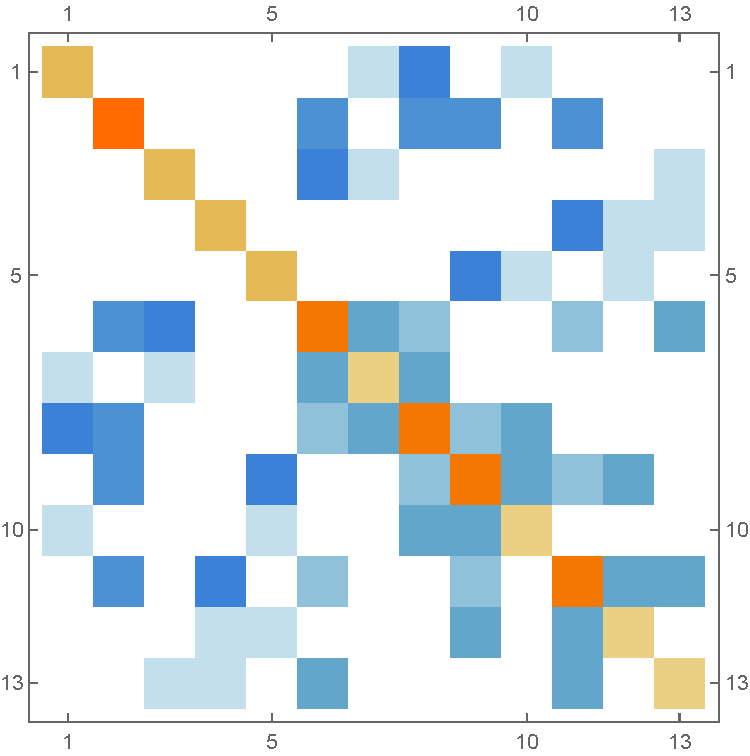
\includegraphics[width=\linewidth]{img/matrixPlotCircle.pdf}
	\caption{Портрет матрицы для рис.~(\ref{fig:matrixPlotCircleMesh})}\label{fig:matrixPlotCircle}
	\endminipage
\end{figure}

\begin{figure}[!hb]
	\minipage{0.4\textwidth}
	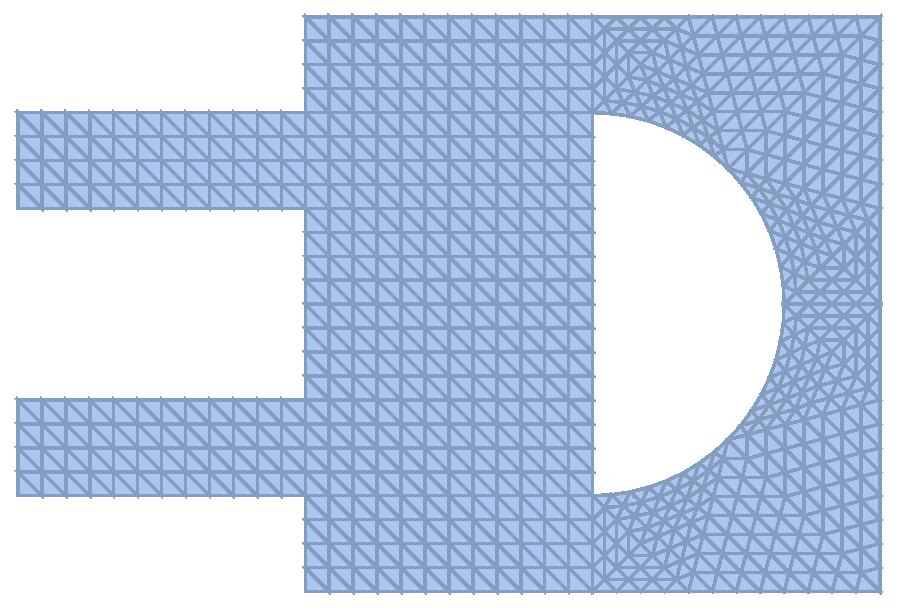
\includegraphics[width=\linewidth]{img/matrixPlotStripsMesh.pdf}
	\caption{Сетка с $n = 800$ для сложной области}\label{fig:matrixPlotStripsMesh}
	\endminipage\hfill
	\minipage{0.4\textwidth}
	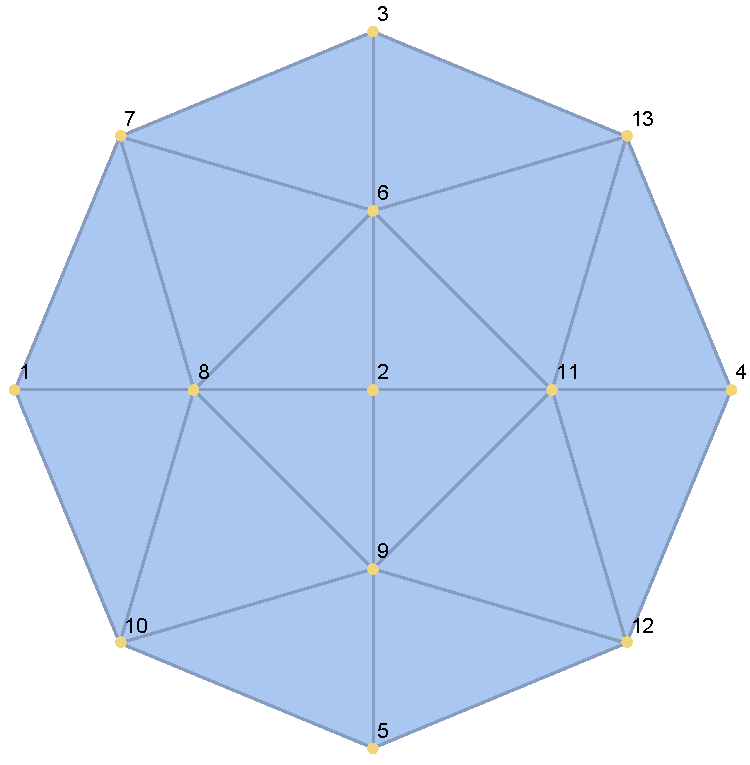
\includegraphics[width=\linewidth]{img/typicalMesh.pdf}
	\caption{Простая триангуляция круга}\label{fig:matrixPlotCircleMesh}
	\endminipage
\end{figure}

Можно показать, что для многих входных в~\ref{stationary} параметров матрица системы $\vect{A}$ будет положительно определена. Поэтому для решения СЛАУ разумно использовать \textbf{метод сопряжённых градиентов} (например, с $\vect{L} \, \vect{D} \, \vect{L}^T$--предобуславливанием).

Подробнее о реализации можно прочесть в~\cite{saad}.






